%==========================================================================%
% MAIN PREAMBLE 
%==========================================================================%
\documentclass[12pt,letterpaper]{report} % Single-sided printing for the library
% \documentclass[12pt,twoside]{report} % Double-sided printing
\usepackage[intlimits]{amsmath}
\usepackage[utf8]{inputenc}
\usepackage{amsfonts,amssymb}
\DeclareSymbolFontAlphabet{\mathbb}{AMSb}
% \usepackage{natbib}
% \usepackage{apalike}
\usepackage{float}
\usepackage[]{caption,subcaption}
\setcaptionmargin{0.5in}
\usepackage{fancyhdr}
%\usepackage{fancyheadings} % what does this do?
\usepackage{fancybox}
\usepackage{ifthen}
\usepackage{template_style} % style package and also some layout stuff
\usepackage{lscape,afterpage}
\usepackage{xspace}
% \usepackage{epstopdf} % what does this do?

\usepackage{appendix}

% https://tex.stackexchange.com/questions/13509/biblatex-in-a-nutshell-for-beginners
% if I get the error, ".bbl not created by bib latex", run biber $, where $ is the basename of the main .tex file, then rerun the build
\usepackage{biblatex}
% \addbibresource{thesis.bib}
% \addbibresource(othersfiles.bib) % if I ever split up the bibiliography add multiple resources like this

%==========================================================================%
%%% graphicx and pdf creation
\usepackage{graphicx}

\usepackage{hyperref} % set up this package last (or almost last anyways)
\hypersetup{
    colorlinks=true,
    linkcolor=red,
    urlcolor=blue,
    citecolor=blue
}

%==========================================================================%
\title{Analysis Note for 60H Dataset Relative Unblinding}
\date{\today}
\author{Nick Kinnaird - Boston University}
%==========================================================================%
% BEGIN
%==========================================================================%
\begin{document}

\maketitle

\chapter*{High Level Summary}

\begin{itemize}
	\item{Lead Analysts: Nick Kinnaird, James Mott}
	\item{Positron Reconstruction Method: Recon West}
	\item{Software Release: V9\_11\_00}
	\item{Dataset: gm2pro\_daq\_full\_run1\_60h\_5033A\_withfullDQC}
	\item{Histogramming Method: Weighted Ratio}
	\item{Gain Correction Method: Default in reconstruction}
	\item{Pileup Correction Method: Asymmetic shadow window, doublets only}
	\item{Lost Muon Spectrum Extraction: Triple coincidence, not included in ratio fit}
	\item{Model for CBO: Exponential envelope, frequency from tracking analysis}
	\item{Model for VW: Exponential envelope, constant frequency, not included in ratio fit}
	\item{Fit Range: $30 \mu s - 500 \mu s$}
	\item{$R = -19.88 \pm 1.373 ppm \pm syst.$ (blinding with common string)}
	\item{$\chi^{2}/NDF = 3052/3145$}
	\item{P value = 0.8806}
\end{itemize}

\textbf{Final fit function:}

\begin{gather*}
		R(t) = \frac{2f(t) - f_{+}(t) - f_{-}(t)}{2f(t) + f_{+}(t) + f_{-}(t)} \\[10pt]
		f_{\pm}(t) = f(t \pm T_{a}/2) \\[10pt]
		f(t) = C(t) (1 + A \cos(\omega_{a}t + \phi)) \\[10pt]
		C(t) = 1 + A_{cbo} e^{-t/\tau_{cbo}} \cos(\omega_{cbo}(t)t + \phi_{cbo})
\end{gather*}
 
\graphicspath{ {Figures/CBO/Frequency/} {Figures/VW/} }

\chapter{Analysis Procedures}
\label{Ch:Procedures}


\section{Key parameters in reconstruction method}

	Default parameters used in the Recon West production of the 60H dataset, with SAM dataset name ``gm2pro\_daq\_full\_run1\_60h\_5033A\_withfullDQC''.

\section{Analysis Data Preparation Procedure}

	\begin{itemize}
		\item{git branch: gm2analyses branch feature/KinnairdAnalyses}
		\item{Majority of code located under gm2analyses/macros/RatioMacro}
	\end{itemize}

	\begin{enumerate}
		\item{Submit jobs to OSG to run the rootTreesAndLostMuons.fcl file which produces root trees of positron hits using the ClusterTree analyzer module and coincident MIP hits using the TestCoincidenceFinder analyzer module.}
		\item{Submit jobs to Fermigrid to produce histograms from root trees using the ClusterTreeToHistsPileup.C macro in RatioMacro/HistMaking. Beyond standard threshold histograms this macro produces pileup and lost muon histograms all within the same root file.}
	\end{enumerate}


\section{Histogramming Procedure}

	Method: Weighted Ratio (threshold)

	\begin{enumerate}
		\item{Loop through all clusters and apply an artificial deadtime (ADT) to combine hits within 6 ns into a single pulse using the same procedure and code that the pileup method uses (see below). Drop clusters with time $< \SI{25}{\mu s}$ or time $> \SI{600}{\mu s}$.}
		\item{Histograms are constructed with ROOT's TH1F class with 149.15 ns bins from $0 - \SI{699.96095}{\mu s}$ corresponding to 4693 bins.}
		\item{Randomize times by $\pm 149.15/2$ ns and fill histograms for energies $> 1.7$ GeV. Randomization uses ROOT's default TRandom3 class.}
		\item{Fill one of the four histograms \{$u_{+}(t), u_{-}(t), v_{1}(t), v_{2}(t)$\} as shown in Equation \ref{eqn:fourHists} per cluster. The associated histogram is determined by generating a random number between 0 and 1, and comparing that number to the relative probabilities of the different weights.}
		\item{Clusters filled into the $u_{+}(t)$ histogram have their times shifted by $t \rightarrow t - T_{a}/2$ and clusters filled into the $u_{-}(t)$ histogram have their times shifted by $t \rightarrow t + T_{a}/2$.}
		\item{$T_{a}$ is known a priori to high precision from the previous experiment, and its value is taken as $1/f_{a}$, where $f_{a}$ is \SI{0.2291}{MHz}:
			\begin{align}
				T_{a} \approx \SI{4.364906}{\mu s}
			\label{eq:Ta}
			\end{align}}
	\end{enumerate}


\section{Gain Correction Procedure}

	Gain correction method: Default by the Italian Calibration Team

	\begin{enumerate}
		\item{Long term gain is corrected using out-of-fill lasers included normalization from the Source Monitor.}
		\item{In-fill gain is corrected using in-fill lasers including normalization from the Source Monitor.}
		\item{Short-term double pulse (SDTP) effect is not included.}
	\end{enumerate}


\section{Pileup Correction Procedure}
\label{Sec:PileupCorrection}

	Pileup correction method: Asymmetric shadow window

	\begin{enumerate}
		\item{Create a vector of clusters per calorimeter per fill. For each cluster look for a second cluster in a window from 12-18 ns after the time of the first cluster. This corresponds to a shadow dead time (SDT) of 6 ns and a shadow gap time (SGT) of 12 ns, equal to 1 and 2 times the applied ADT respectively.}
		\item{Create shadow doublets with energies and times as:
			\begin{gather}
				E_{doublet} = C \cdot (E_{1} + E_{2}), \\
				t_{doublet} = \frac{t_{1} \cdot E_{1} + (t_{2}-SGT) \cdot E_{2}}{E_{1} + E_{2}},
			\end{gather}
		where the latter equation is just the energy-weighted time between the two singlets. In the former equation, the calculation of the doublet energy is the sum of the singlets times some factor. That factor is set equal to 1, which is a decent approximation since the spatial separation in the reconstruction is turned off, and because the Short Term Double Pulse (SDTP) improvement to the laser energy calibration will be applied. The systematic effects of a factor not equal to 1 are studied in Section \ref{SubSec:PileupPhase}.}
		\item{Randomize $t_{doublet}$ times by $\pm 149.15/2$ ns as in the histogramming procedure described above.}
		\item{For each calorimeter construct a pileup spectrum P = doublets - singlets = D - S, where the singlets are subtracted at time $t_{doublet}$ as opposed to their individual times, and pulses are only added or subtracted if they are above 1.7 GeV. Subtract P off energy and threshold histograms.}
		\item{For pileup subraction in the ratio method, randomly split associated doublets and singlets into 4 separate histograms as is done in the histogramming procedure described above, with times shifted accordingly. Subtract 4 pileup histograms off corresponding \{$u_{+}(t), u_{-}(t), v_{1}(t), v_{2}(t)$\} histograms before forming the ratio.}
		\item{The errors of the pileup corrected histogram were determined to be: 
			\begin{gather}
				\sigma(N_{corrected}) = \sqrt{N_{corrected} + 2 N_{1} + 6 N_{4}},
			\end{gather}
		where $N_{1}$ is the number of doublets where both singlets were below threshold, and $N_{4}$ is the number of doublets where both singlets were above threshold, and this is a quantity evaluated at each time bin. (Cite this? DocDB 14830. Derive this in the appendix?) A histogram of error multipliers was created by factoring out the $N_{corrected}$ term, which is then applied to the bin errors before fitting. This is true even for the ratio errors to good approximation. (Cite this? Derive it as JP did?) Note that I did not time randomize the $N_{1}$ and $N_{4}$ entries when constructing the correct errors, which should have a negligble effect.}
		\item{The pileup correction at the triplet/contamination level is not included. The machinery exists to apply such a correction, but it requires more work to get it correct. It has been determined not be necessary for the 60H and Run 1 data.}
	\end{enumerate}


\section{Lost muon spectrum extraction procedure}

	Method: Triple coincidence of clusters

	Note that the lost muons are not included in the ratio fit because the ratio method divides out such slow effects. This is reflected by the lack of a low frequency peak in the FFT of the fit residuals for the ratio fit, whereas such a peak exists for T method fits. I include here however my method for extracting the lost muon function for possible future systematic studies.

	\begin{enumerate}
		\item{Triple coincidence of clusters in 3 consecutive calorimeters are made with an energy cut of 100 MeV $<$ E $<$ 250 MeV and 5 ns $<$ dt $<$ 8.5 ns.}
		\item{A time histogram is made with the muon cluster in the first calorimeter.}
		\item{The function that would be used in the final fit is:
			\begin{gather}
				\Lambda(t) = 1 - \kappa_{loss} \int_{0}^{t} L(t')e^{(-t'/\gamma\tau_{\mu})} dt'
			\end{gather}
		where $L(t)$ is the triples histogram, and an arbitrary $10^{-6}$ factor has been absorbed into $\kappa_{loss}$ in order to bring it to a more reasonable value (from $\mathcal{O}(10^{-10})$ to $\mathcal{O}(10^{-4})$).}
	\end{enumerate}


\section{Beam Dynamics: CBO Model}
\label{Sec:CBO}

	\begin{enumerate}
		\item{The CBO frequency as a function of time is taken from the tracking analysis, DocDB 14208, and shown in Figure \ref{fig:TrackerCBOModel}. The CBO frequency is not constant because the quad voltage was not constant as a function of time. As described in that document, the source of this is almost certainly the fact that some of the quad resistors were damaged, leading to longer RC time constants. The form used is 
			\begin{gather}
				\omega_{cbo}(t) = \omega_{0}(1 + \Delta\omega t + A e^{-t/\tau_{A}} + B e^{-t/\tau_{B}}),
			\end{gather}
		with parameters determined from station 12 in the 60H dataset and fixed in the fit as:
			\begin{equation*}	
			\begin{aligned}
			 	\Delta\omega &= \SI{1.86e-8}{ns^{-1}}, \\
			 	A &= -0.0504, \\
			 	\tau_{A} &= \SI{73.3}{\mu s}, \\
			 	B &= -0.131, \\
			 	\tau_{B} &= \SI{16.6}{\mu s}. \\
			\end{aligned}
			\end{equation*}
		The parameter $\omega_{0}$ is allowed to float in the fit and starts with a value of $\SI{2.3051}{rad.\mu s^{-1}}$. The ratio method has trouble with letting the other parameters float, and fixing them to slightly different values does not change the fit results significantly. Parameter values determined from station 18 are similar to those from station 12 and were also tested with no significant change in the fit results.}
		\item{Because the ratio method divides out the CBO partially (reduction by a factor of $\sim5$ in the FFT cbo peak amplitude), the ratio fit has a hard time fitting the CBO lifetime. Therefore $\tau_{cbo}$ is fixed to $\SI{180}{\mu s}$, determined from a T Method fit to the same data.}
		\item{An exponential function is assumed for the CBO decoherence.}
		\item{The $N_{cbo}$ term is included in the fit, $A_{cbo}$ and $\phi_{cbo}$ are excluded. The 2CBO term is excluded.}
		\item{The final CBO function is:
			\begin{gather}
					N_{cbo}(t) = C(t) = 1 + A_{cbo} e^{-t/\tau_{cbo}} \cos(\omega_{cbo}(t)t + \phi_{cbo})
			\label{eqn:CBO}
			\end{gather}
		}
	\end{enumerate}

	\begin{figure}[]
		\centering
		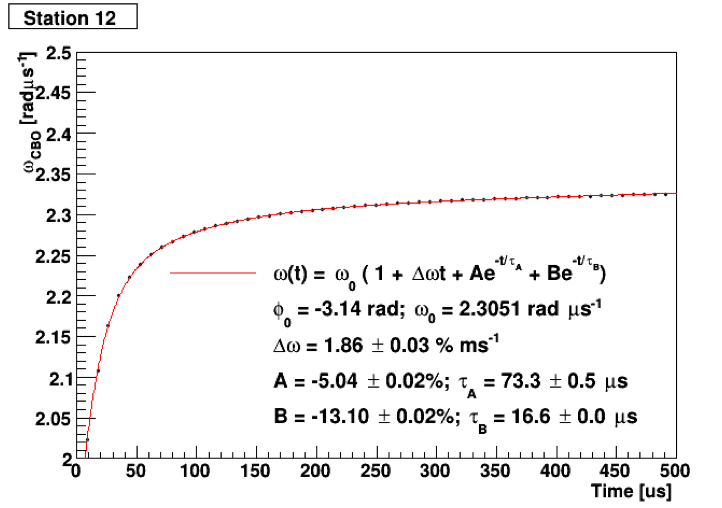
\includegraphics[width=\textwidth]{TrackerCBOModel}
	    \caption[TrackerCBOModel]{Plotted is the CBO frequency determined with tracker data as a function of time, for station 12 in the 60H dataset. The frequency was modeled as a sum of a constant with a linear part and two exponentials. It rises sharply at early times and slowly over the rest of the fill. Plot created by James Mott.}
	    \label{fig:TrackerCBOModel}
	\end{figure}


\section{Beam Dynamics: Vertical Waist Model}
\label{Sec:VW}

	\begin{enumerate}
		\item{\wa is senstive to the width of the beam, which is characterized by the frequency 
			\begin{gather}
				f_{VW} = f_{cyc} - 2f_{y}, \\
				f_{y} = f_{cbo} \sqrt{\frac{2f_{cyc}}{f_{cbo}} - 1}.
			\end{gather}}
		\item{An exponential function is assumed for the VW decoherence as in the CBO, and so the VW term is defined as
			\begin{gather}
					V(t) = 1 + A_{VW} e^{-t/\tau_{VW}} \cos(\omega_{VW}t + \phi_{VW})
			\end{gather}
		}
		\item{$\omega_{VW}$ is assumed to be a constant value even though the CBO frequency changes vs time.}
	\end{enumerate}

	In the 60H dataset $f_{VW} \approx \SI{2.3}{MHz} \approx 10 \cdot \omega_{a}$, which is an even multiple of the \gmtwo frequency. It turns out that any frequencies which are even multiples of the \gmtwo frequency largely cancel in the ratio. This is shown for the vertical waist in Figure \ref{fig:VWPlot}. This combined with the time randomization to remove the fast rotation ($f_{cyc}$) means the vertical waist does not need to be included in the ratio fit. This is justified by the lack of a vertical waist peak in the FFT of the residuals of the fit, as will be shown later.

	\begin{figure}[]
		\centering
		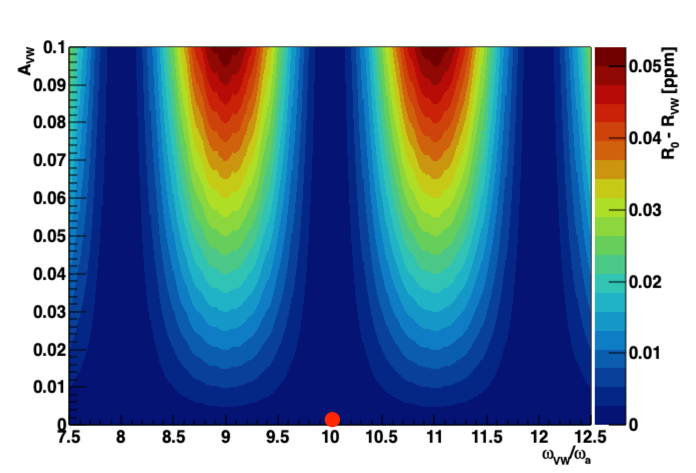
\includegraphics[width=\textwidth]{VWPlot}
	    \caption[VWPlot]{Plotted is the difference in the maximum value of the ratio with a vertical waist function included and without, as a function of both the amplitude of the vertical waist effect and the vertical waist frequency in units of the \gmtwo frequency. This was created with a toy Monte Carlo. As is shown the difference reaches a minimum for even multiples of the \gmtwo frequency. The 60H dataset lives at the bottom center of this plot, where the difference in the ratio is approximately \SI{5e-6}{} at 30 $\mu s$. Plot created by James Mott.}
	    \label{fig:VWPlot}
	\end{figure}


\section{Final Fit Function}
\label{Sec:FinalFitFunction}

	The following function is used for the final fit for each calorimeter and for the calorimeter sum:
	\begin{gather}
			R(t) = \frac{2f(t) - f_{+}(t) - f_{-}(t)}{2f(t) + f_{+}(t) + f_{-}(t)} \\[10pt]
			f_{\pm}(t) = f(t \pm T_{a}/2) \\[10pt]
			f(t) = C(t) (1 + A \cos(\omega_{a}t + \phi)) \\[10pt]
			C(t) = 1 + A_{cbo} e^{-t/\tau_{cbo}} \cos(\omega_{cbo}(t)t + \phi_{cbo}) \\[10pt]
			\omega_{a} = 2 \pi \cdot \SI{0.2291}{MHz} \cdot (1 + R \times 10^{-6})
	\end{gather}
	All parameters are floating except for terms in $\omega_{cbo}(t)$ and $\tau_{cbo}$ as described above.



 



\begin{appendices}
Should my appendix really be a section at the front of the report? Or should it be in the appendix as I've place it here?

\chapter{Ratio Method Derivation and Fit Function}

Consider the 5 parameter function:
	\begin{align}
		N_{5}(t) = N_{0}e^{-t/\tau}(1 + A \cos(\omega_{a}t + \phi)),
	\end{align}
which describes some ideal dataset in histogram format. Here $\phi$ will be set to zero for simplicity. Now define the variables $u_{+}(t)$, $u_{-}(t)$, $v_{1}(t)$, and $v_{2}(t)$ as
	\begin{equation}
	\begin{aligned}
		u_{+}(t) &= \frac{1}{4} N_{5}(t+T/2) \\
		u_{-}(t) &= \frac{1}{4} N_{5}(t-T/2) \\
		v_{1}(t) &= \frac{1}{4} N_{5}(t) \\
		v_{2}(t) &= \frac{1}{4} N_{5}(t),
	\end{aligned}
	\end{equation}
where the $1/4$ out front reflects randomly splitting the whole dataset into 4 equally weighted sub-datasets, and T is the g-2 period known to high precision, $\mathcal{O}(10^{-6})$. This corresponds to a weighting of 1:1:1:1 between the datasets. To be explicit here regarding the signs, the counts that are filled into the histogram described by $u_{+}$ have their times shifted as $t \rightarrow t - T/2$, which is what the function $N_{5}(t+T/2)$ describes, and vice versa for $u_{-}$. To form the ratio define the variables:
	\begin{equation}
	\begin{aligned}
		U(t) &= u_{+}(t) + u_{-}(t) \\
		V(t) &= v_{1}(t) + v_{2}(t) \\
		R(t) &= \frac{V(t) - U(t)}{V(t) + U(t)}.
	\end{aligned}
	\end{equation}
Plugging in and dividing the common terms $(N_{0}e^{-t/\tau}/4)$,
	\begin{align}
		R(t) = \frac{2(1 + A \cos(\omega_{a}t)) - e^{-T/ 2\tau} (1 + A \cos(\omega_{a}t + \omega_{a}T/2)) - e^{T/ 2\tau} (1 + A \cos(\omega_{a}t - \omega_{a}T/2))} {2(1 + A \cos(\omega_{a}t)) + e^{-T/ 2\tau} (1 + A \cos(\omega_{a}t + \omega_{a}T/2)) + e^{T/ 2\tau} (1 + A \cos(\omega_{a}t + \omega_{a}T/2))}.
	\end{align}

Now set $\omega_{a}T/2 = \delta$, and note that T is really
	\begin{equation}
	\begin{aligned}
 		T = T_{guess} = \frac{2\pi}{\omega_{a}} + \Delta T, \\
 		\Delta T = T_{guess} - T_{true}.
	\end{aligned}
	\end{equation}
Being explicit, 
	\begin{align}
		\delta = \frac{\omega_{a}}{2} T_{guess} = \frac{\omega_{a}}{2} (\frac{2\pi}{\omega_{a}} + \Delta T) = \pi + \pi \frac{\Delta T}{T_{true}} = \pi + \pi (\delta T),
	\end{align}
and $\delta$ can be redefined as 
	\begin{align}
		\delta = \pi (\delta T),
	\end{align}
by flipping the sign of any cosine terms that contain $\delta$.

Then, using the trig identity 
	\begin{align}
		\cos(a \pm b) = \cos(a)\cos(b) \mp \sin(a)\sin(b)
	\end{align}
so that 
	\begin{equation}
	\begin{aligned}
		\cos(\omega_{a}t \pm \delta) &= \cos(\omega_{a}t)\cos{\delta} \mp \sin(\omega_{a}t)\sin{\delta} \\
		&\approx \cos(\omega_{a}t)(1-\delta^{2}) \mp \sin(\omega_{a}t)\delta \\
		&\approx \cos(\omega_{a}t),
	\label{eqn:trig}
	\end{aligned}
	\end{equation}
since $\delta \sim O(10^{-5})$, the ratio becomes
	\begin{align}
		R(t) \approx \frac{2(1 + A \cos(\omega_{a}t)) - (1 - A \cos(\omega_{a}t))(e^{-T/ 2\tau} + e^{T/ 2\tau})} {2(1 + A \cos(\omega_{a}t)) + (1 - A \cos(\omega_{a}t))(e^{-T/ 2\tau} + e^{T/ 2\tau})}.
	\end{align}
Expanding
	\begin{align}
		e^{\pm T/ 2\tau} = 1 \pm \frac{T}{2\tau} + \frac{1}{2} \Big(\frac{T}{2\tau}\Big)^{2} \pm \dots,
	\end{align}
repacing and simplifying,
	\begin{align}
		R(t) \approx \frac{A \cos(\omega_{a}t) - C (1 - A \cos(\omega_{a}t))}{1 + C (1 - A \cos(\omega_{a}t))},
	\end{align}
where
	\begin{align}
		C = \frac{1}{16} \Big(\frac{T}{\tau}\Big)^{2} \approx 2.87 * 10^{-4}.
	\end{align}

Using the expansion 
	\begin{align}
		f(x) = \frac{1}{1+x} = 1 - x + x^2 - \dots, \quad |x| < 1,
	\end{align}
and since $C$ is small, the denominator can be manipulated such that
	\begin{equation}
	\begin{aligned}
		R(t) &\approx (A \cos(\omega_{a}t)) - C (1 - A \cos(\omega_{a}t)))(1 - C (1 - A \cos(\omega_{a}t))) \\
		     &\approx A \cos(\omega_{a}t) - C + C A^{2} \cos^2(\omega_{a}t),
	\end{aligned}
	\end{equation}
after dropping terms of $\mathcal{O}(C^{2})$ and higher. In practice the last term is ommitted since it has a minimal effect on the fitted value of $\omega_{a}$ \cite{cite}, and one arrives at
	\begin{align}
		R(t) \approx A \cos(\omega_{a}t) - C,
	\end{align}
the conventional 3 parameter ratio function.


In order to avoid approximations one can instead weight the counts in the histograms as
	\begin{align}
		u_{+}(t) : u_{-}(t) : v_{1}(t) : v_{2}(t) = e^{T/2\tau} : e^{-T/2\tau} : 1 : 1,		
	\end{align}
so that
	\begin{equation}
	\begin{aligned}
		u_{+}(t) &= \frac{e^{T/2\tau}}{2 + e^{T/2\tau} + e^{-T/2\tau}} N_{5}(t+T/2) \\
		u_{-}(t) &= \frac{e^{-T/2\tau}}{2 + e^{T/2\tau} + e^{-T/2\tau}} N_{5}(t-T/2) \\
		v_{1}(t) &= \frac{1}{2 + e^{T/2\tau} + e^{-T/2\tau}} N_{5}(t) \\
		v_{2}(t) &= \frac{1}{2 + e^{T/2\tau} + e^{-T/2\tau}} N_{5}(t).
	\label{eqn:fourHists}
	\end{aligned}
	\end{equation}
(These factors out front aren't so far off from 1/4 since $e^{\pm T/ 2\tau} \approx e^{\pm 4.35/ 2*64.4} \approx 1.034, .967$.) Then instead $R(t)$ becomes 
	\begin{align}
		R(t) = \frac{2(1 + A \cos(\omega_{a}t)) - (1 - A \cos(\omega_{a}t + \delta)) - (1 - A \cos(\omega_{a}t - \delta))} {2(1 + A \cos(\omega_{a}t)) + (1 - A \cos(\omega_{a}t + \delta)) + (1 - A \cos(\omega_{a}t + \delta))},
	\end{align}
where the $e^{\pm T/ 2\tau}$ terms out front now cancel. Using Equation \ref{eqn:trig} again and this time avoiding approximations in $\delta$,
	\begin{align}
		R(t) = \frac{2A \cos(\omega_{a}t) (1 + \cos{\delta} )} {4 + 2A \cos(\omega_{a}t) (1 - \cos{\delta} )},
	\end{align}
after simplifying. In the limit that 
	\begin{align}
		\delta = \pi (\delta T) \rightarrow 0
	\end{align}
since $\delta T$ is small, 
	\begin{align}
		R(t) \approx A \cos(\omega_{a}t),
	\end{align}
with the only approximation being made at $\mathcal{O}(\delta^{2}) \sim \mathcal{O}(10^{-10})$.

Finally, while the 3 parameter ratio function suffices for fits to data containing slow modulations, it does not suffice for faster oscillation features. In that case it is more useful to fit with the non-approximated or simplified version of the ratio,
	\begin{equation}	
	\begin{aligned}
		R(t) &= \frac{v_{1}(t) + v_{2}(t) - u_{+}(t) - u_{-}(t)}{v_{1}(t) + v_{2}(t) + u_{+}(t) + u_{-}(t)}, \\ 
			 &= \frac{2f(t) - f_{+}(t) - f_{-}(t)}{2f(t) + f_{+}(t) + f_{-}(t)},
	\end{aligned}
	\end{equation}
where
	\begin{equation}	
	\begin{aligned}
		f(t) &= C(t) (1 + A \cos(\omega_{a}t + \phi)) \\ 
		f_{\pm}(t) &= f(t \pm T_{a}/2),
	\end{aligned}
	\end{equation}
and $C(t)$ can encode any other effects in the data that need to be fitted for, such as the CBO,
	\begin{align}
		C(t) = 1 + A_{cbo} e^{-t/\tau_{cbo}} \cos(\omega_{cbo}t + \phi_{cbo}).
	\end{align}
Additionally, any other fit parameters such as $A$ or $\phi$ can be made a fuction of $t$. Using the non-approximated form for the final fit function gives greater confidence in the fit results for the high precision $\omega_{a}$ extraction necessary for the experimental measurement.


\chapter{Ratio Method Errors}

\end{appendices}


%==========================================================================%
\end{document}
